\documentclass[thesis.tex]{subfiles}
\begin{document}

\chapter{Introduction}
\label{chap:introduction}

\begin{figure}[h]
\centering
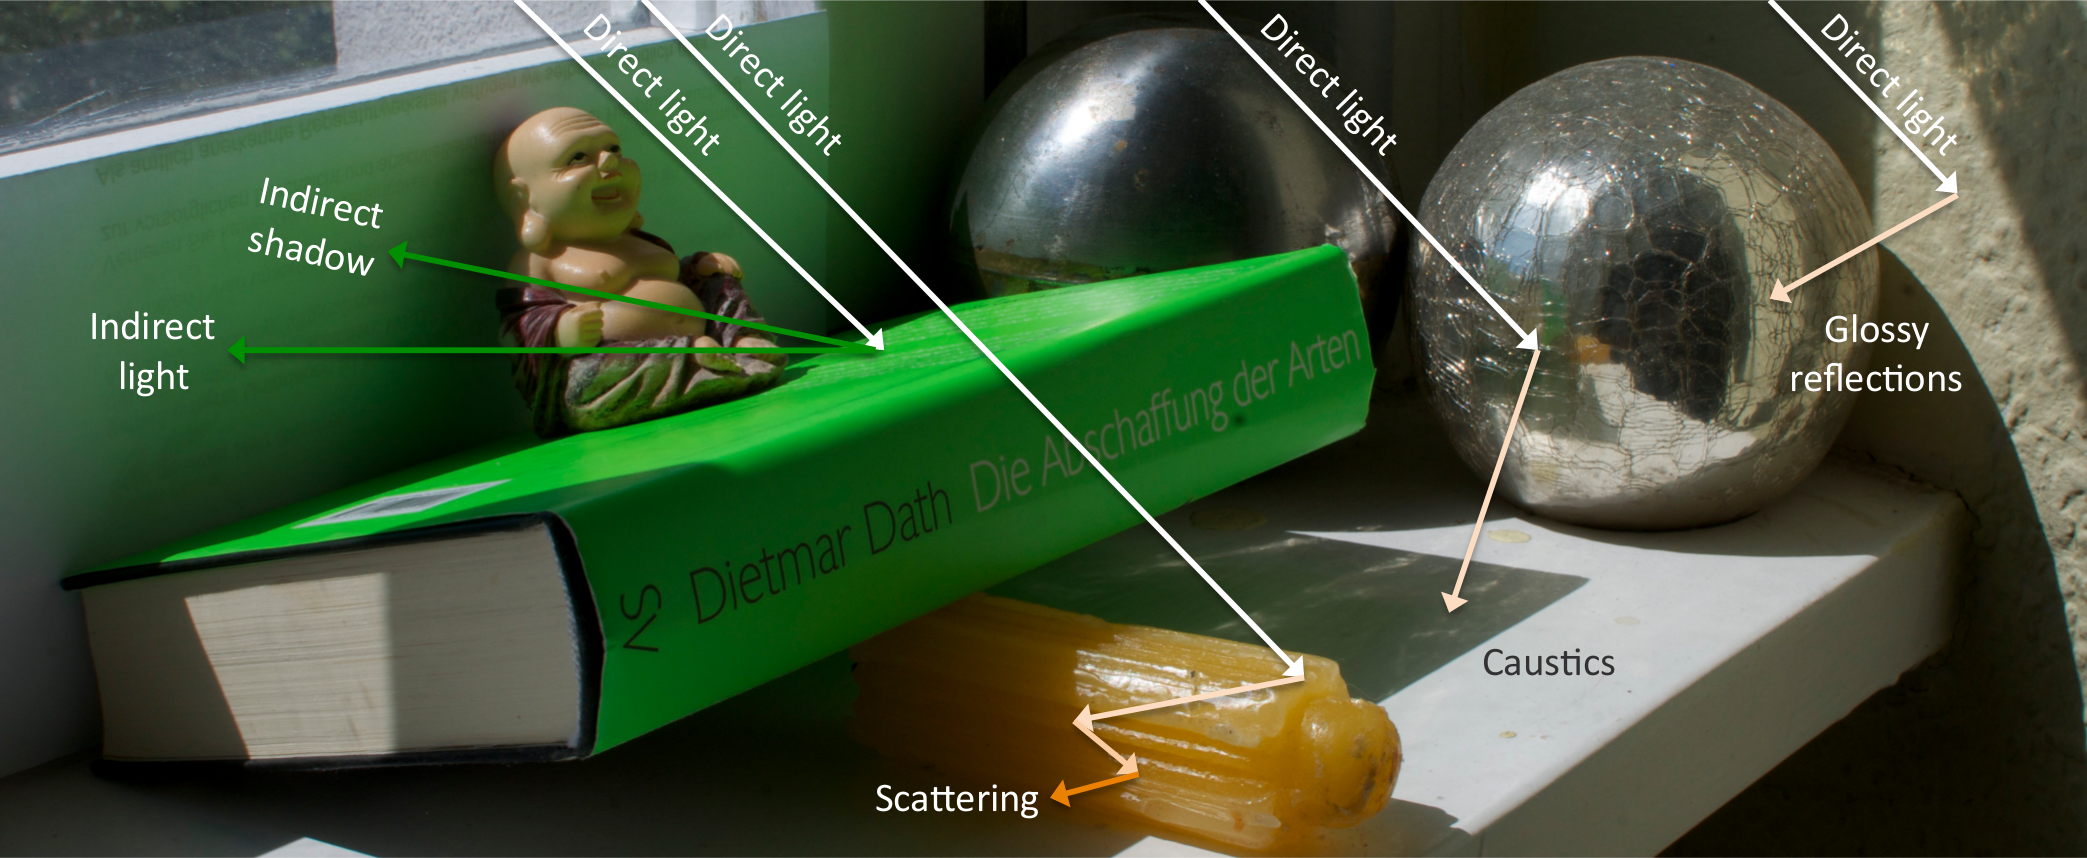
\includegraphics[width=\textwidth]{giphenomenons}
\caption{\cite{bib:RealtimeGIOverview} Photography of a scene with global illumination: Diffuse and specular bounces, caustics and scattering.}
\label{fig:giphenomenons}
\end{figure}

\section{Introduction}
Everything that human eyes can perceive is the result of light originating from a source, interacting with matter and finally reaching the retina.
The way how light interacts with our environment is very complex and depends always on a global context:
There is a variety of natural phenomenons like shadowing, light bleeding, glossy reflections, and scattering which are impossible to simulate by local lighting models.
The Photography in \autoref{fig:giphenomenons} demonstrates a few of them.
Compared to the simulation of local light effects which only take an isolated surface point into consideration, the simulation of global illumination effects as they occur in nature are extremely challenging both in terms of computational and algorithmic complexity.
\\
Simulated scenes which lack these global effects look synthetic and are often missing important cues which are needed to understand interrelations of objects.
Wherever 3D-scenes need to be displayed in a either believable or aesthetic manner, the simulation of global illumination becomes important.
Some of these applications are namely visual effects in (or even entire) movies, architectural visualizations video games and professional training simulations.
While the demands of these applications vary greatly, the underlying principles are the same as they are governed by the physical laws of light to which our visual system is used to.
\\
Generally, these applications can be divided in two categories: Interactive and non-interactive.
Where a non-interactive application like a movie or single images can easily have computation times of many days, interactive applications need to compute at least parts of the simulation just in time to provide the user with the expected feedback on his actions.
A simulation is usually called interactive if images are rendered in less than 50ms (20 frames per second).
However frame rates need to be much higher to be comfortable for the user.
Fast paced games usually profit usually from high rendering times of 16ms (about 60 frames per second) \cite{bib:shooterfps} and the vendors of the upcoming virtual reality displays recommend even shorter rendering times of 11-8ms (90-120 frames per second) to reduce motion sickness \cite{bib:oculushighfps} \todo{another reference to another vender would be nice}.
Naturally, real-time rendering that is performed on personal computers usually makes use of a different set of approaches and algorithms as offline rendering which runs often on larger computer clusters.
In this work we concentrate exclusively on real-time rendering without any pre-computation.
% resolutions rising?

\section{Motivation}
\begin{figure}[h]
\centering
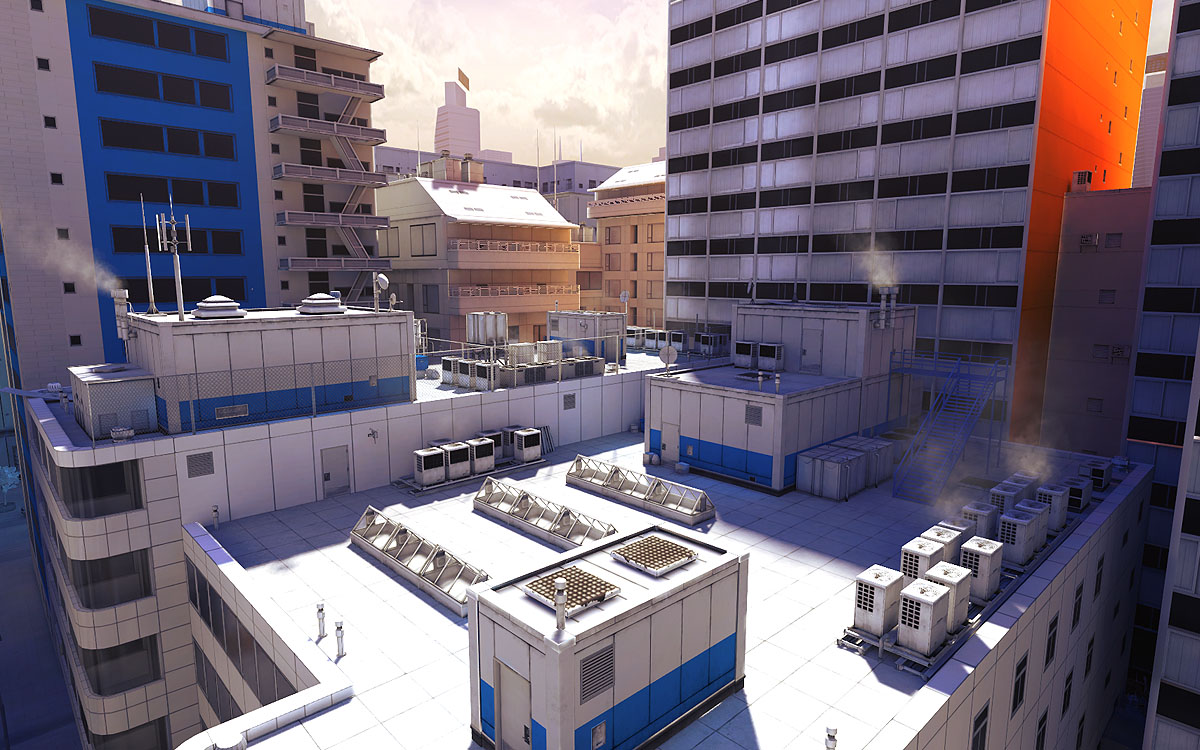
\includegraphics[width=\textwidth]{mirrorsedgescreenshot}
\caption{Screenshot from the 2008 video game \emph{Mirrors Edge}, featuring precomputed indirect lighting.}
\label{fig:gameprecomputedgi}
\end{figure}
To be able to display the aforementioned light effects in real-time, interactive application make often use of various pre-computation steps under the assumption that specific parts of the scene do not change.
In the extreme case this means that both scene and lighting conditions are assumed to be completely static which allows to compute a large variety of effects up-front.
This is common practice in many games, as seen e.g. in Mirrors Edge in \autoref{fig:gameprecomputedgi} where only the characters and very few dynamic objects are lit at runtime.
\\
Obviously such techniques imply many restrictions on the design of virtual worlds and may not be applicable at all.
However, there are also solutions which less restrictions, for example precomputed light transport techniques that allow dynamic lights in a static scene or irradiance volumes which can apply precomputed lighting on dynamic objects (more on other techniques in \autoref{chap:prevwork}).
Of course there are various trade-offs between different approaches and so far there is no technique that is close to simulate all global illumination effects in real-time at reasonable quality (which is also still an open problem for offline rendering).
\\
TODO: stress how great it would be to have fully dynamic GI and lead over to what we actually want to achieve


\section{Goals}
\begin{itemize}
\item Realtime global illumination, first bounce
\subitem Dynamic camera, scene and lights!
\item No significant precomputation
\subitem This is important, as it excludes LightSkin!
\item Support both diffuse and glossy reflections
\subitem Simple BRDFs are okay, but we want to parameterize them 
\item Temporal consistency
\item Preferable scalable with large scenes
\item Adequate lighting quality
\item Colored indirect shadows
\subitem Obviously I need to make a heavy trade-off here
\end{itemize}

\section{Overview}
todo: This paragraph is a compressed version of the main part

\section{Thesis Outline}
todo

\subfilebib % Makes bibliography available when compiling as subfile
\end{document}